\documentclass[conference]{IEEEtran}
\IEEEoverridecommandlockouts

\usepackage{cite}
\usepackage{amsmath,amssymb,amsfonts}
\usepackage{algorithmic}
\usepackage{graphicx}
\usepackage{textcomp}
\usepackage{xcolor}
\usepackage{booktabs}
\usepackage{url}

\begin{document}

\title{Adaptive Behavioral Deception-Resistant Insider Threat Detection Using Counterfactual Digital Twins}

\author{
\IEEEauthorblockN{Dr. RAJENDRAN T}
\IEEEauthorblockA{\textit{Department of CSE, Cyber Security} \\
\textit{Vel Tech Rangarajan Dr. Sagunthala R\&D Institute of Science and Technology} \\
Chennai 600062, India \\
TTS3844 \\
devajendrant@veltech.edu.in}
\and
\IEEEauthorblockN{Haritha D}
\IEEEauthorblockA{\textit{Department of CSE, Cyber Security} \\
\textit{Vel Tech Rangarajan Dr. Sagunthala R\&D Institute of Science and Technology} \\
Chennai 600062, India \\
VTU24553 \\
vtu24553@veltech.edu.in}
\and
\IEEEauthorblockN{Mahisha V}
\IEEEauthorblockA{\textit{Department of CSE, Cyber Security} \\
\textit{Vel Tech Rangarajan Dr. Sagunthala R\&D Institute of Science and Technology} \\
Chennai 600062, India \\
VTU25143 \\
vtu25143@veltech.edu.in}
}

\maketitle

\begin{abstract}
Internal security breaches present a stubborn defensive dilemma because authenticated personnel already hold valid login credentials and legitimate file privileges. Static rule correlations in standard security information management deployments miss nuanced, low-volume exfiltration, whereas unconstrained self-updating machine learning baselines remain vulnerable to baseline poisoning, where an insider intentionally paces illicit activity over weeks so that the learning algorithm gradually adopts malicious volumes as ordinary background behaviour. In this work, we build an end-to-end insider risk detection framework combining low-level Windows kernel interrogation, unsupervised Isolation Forest scoring, and a Counterfactual Digital Twin sandbox. Telemetry on our testbed host captures live process launches, delta transmission bytes, and physical flash drives verified via the Win32 GetDriveTypeW function, entirely bypassing spoofed network mounts. We project user telemetry into a six-dimensional orthogonal vector and track normalized baseline divergence. Whenever cumulative drift reaches or exceeds 4.5, a Persistence Drift-Lock engages, instantly freezing baseline updates so malicious actions cannot contaminate normal models. Simultaneously, our Counterfactual Digital Twin lets security operators perturb behavioral features to evaluate how minute adjustments in user habits alter risk scores. In a rigorous benchmark of 170 recorded operational scenarios comprising 90 deliberate multi-vector attacks and 80 normal business activities, our prototype caught 82 of 90 attacks, yielding a 91.11\% recall rate, a 93.18\% precision rate, an F1-score of 0.9213, and a false positive rate of 7.50\% across 6 false alarms. These empirical findings substantiate that linking kernel-level hardware verification with locked isolation ensembles effectively counters slow behavioral poisoning while keeping investigation workflows transparent.
\end{abstract}

\begin{IEEEkeywords}
Insider threat detection, behavioral analysis, anomaly detection, concept drift, deception resistance, counterfactual digital twin, Isolation Forest.
\end{IEEEkeywords}

\section{Introduction}

\subsection{Background}
Modern enterprise networks depend heavily on distributed infrastructure to house sensitive corporate intellectual property, employee records, and client financial data. While perimeter defensive walls successfully deflect external intrusion attempts, internal operators already possess cryptographic keypairs, domain authorizations, and direct visibility into corporate repositories. Malicious employees, compromised administrator tokens, and disgruntled personnel exploit this established trust boundary to pull data out without tripping standard perimeter alarms \cite{b1}, \cite{b2}.

Distinguishing malicious operations from routine administrative duties remains difficult because an identical event can represent either legitimate business or serious industrial espionage depending entirely on context \cite{b3}. A 2.5 GB compressed file archive sent offsite could simply be an approved weekend disaster recovery backup, or it could represent a catastrophic data exfiltration event. Seasoned insiders leverage this ambiguity through sophisticated operational evasion tactics, such as low-and-slow data exfiltration where files are throttled to blend with normal traffic, off-hours staging where archives are compiled during night shifts to escape supervision, and baseline poisoning, often described as a boiling frog attack, where an attacker slowly increases transfer sizes so adaptive systems accept high data movements as normal baseline habits \cite{b4}, \cite{b5}.

Signature-based firewalls, host intrusion systems, and static security alerts fail against these tactics because the actor utilizes authorized credentials. Unsupervised anomaly models detect statistical deviations without requiring pre-labeled attack sets \cite{b6}, \cite{b7}. However, when these models self-tune continuously on unverified daily telemetry, an adversary can deliberately contaminate the baseline, rendering the detector blind.

This research introduces an insider threat detection architecture that unites continuous hardware-level host monitoring, unsupervised Isolation Forest scoring, and a multi-attribute drift lock to stop baseline poisoning before it starts. We also build a Counterfactual Digital Twin sandbox allowing analysts to simulate what-if adjustments in employee routines, making automated threat scoring explainable and defensible.

\subsection{Problem Statement}
Existing user and entity behavior analytics platforms stumble across two primary architectural hurdles. First, adaptive models struggle to differentiate harmless operational changes from deliberate adversarial concept drift. A completely static baseline triggers excessive false positives when an employee workload expands. Conversely, sliding-window models or exponential moving averages absorb slow attack escalation into the running baseline, normalizing the attack \cite{b5}, \cite{b8}.

Second, current detection platforms offer very poor counterfactual visibility. An alert indicates that an anomaly happened, but fails to explain what specific actions caused the spike or how an employee behavior would have looked under safe, normative conditions. Without counterfactual reasoning, security operations analysts waste critical hours manually piecing together evidence from fragmented system logs.

Addressing these vulnerabilities requires a system that correlates low-level hardware indicators across multiple orthogonal feature dimensions, halts baseline adaptation when suspicious shifts occur, and provides a simulation sandbox for investigating alternative behavioral scenarios.

\subsection{Objectives and Contributions}
Our research accomplishes four practical engineering objectives:
\begin{enumerate}
    \item Kernel-Verified Endpoint Sensor: We build a lightweight background agent that extracts active process hierarchies, delta transmission throughput via psutil, and verifies physical USB mass storage by calling the Win32 GetDriveTypeW function directly, confirming return code 2 to prevent synthetic drive confusion.
    \item Persistence Drift-Lock Defense: We couple an unsupervised Isolation Forest configured with 100 trees and 600 baseline samples with a cumulative Z-score metric. When composite multi-vector deviation reaches or exceeds 4.5, our persistence lock immediately halts baseline updates, shielding the model from poisoning.
    \item Interactive Counterfactual Digital Twin Sandbox: We implement a simulation interface that mirrors employee behavioral baselines, letting analysts manipulate login times, file access counts, outbound network volumes, and USB peripherals to evaluate how specific adjustments impact overall risk.
    \item Decoupled Enterprise Architecture: We organize the prototype into four distinct tiers comprising a host monitoring daemon, a Node.js and Express API gateway on port 5000, a Python Flask machine learning service on port 5001, and a React 18 dashboard on port 3000 backed by MongoDB storage.
\end{enumerate}

\begin{table}[htbp]
\caption{Qualitative Comparison of Detection Approaches}
\label{tab:approaches}
\centering
\resizebox{\columnwidth}{!}{%
\begin{tabular}{lll}
\toprule
\textbf{Approach} & \textbf{Core Strength} & \textbf{Operational Limitation} \\
\midrule
Rule-based detection & Straightforward policy enforcement & Vulnerable to low-and-slow evasion \\
Naive adaptive ML & Absorbs benign shifts dynamically & Vulnerable to baseline poisoning \\
Static Isolation Forest & Immune to baseline contamination & High false alarms under benign shifts \\
\textbf{Proposed Framework} & \textbf{Drift-locked Isolation Forest with Twin} & \textbf{Requires initial baseline calibration} \\
\bottomrule
\end{tabular}%
}
\end{table}

Table \ref{tab:approaches} summarizes how our proposed strategy compares against conventional methods. While fixed rules excel at catching overt violations, they crumble when faced with paced transfers. Naive self-tuning algorithms handle natural workflow evolution but expose the organization to baseline poisoning. Static anomaly detectors prevent contamination but trigger unsustainable false alarm rates. Our framework bridges this operational gap by maintaining an adaptive state that freezes under anomalous divergence, combining high detection fidelity with stability.

\section{Related Work}

\subsection{Endpoint Heuristics and Anomaly Baselines}
Early enterprise endpoint defenses depended primarily on rigid signature heuristics and static threshold policies \cite{b3}, \cite{b4}. While such mechanisms reliably flag explicit operational violations, such as single-burst copies exceeding bulk transfer limits, they prove ineffective against deliberate adversaries who throttle file transfers below programmed alerting limits \cite{b8}, \cite{b9}.

To overcome fixed threshold weaknesses, security research turned toward data-driven user and entity behavior analytics. Unsupervised statistical paradigms, particularly tree-partitioning isolation heuristics and hyperplane boundary estimators, identify irregular outliers without requiring pre-labeled attack repositories \cite{b6}, \cite{b7}. By recursively slicing random feature intervals, anomalies are isolated close to tree root partitions. Nevertheless, static anomaly detectors cannot distinguish between harmless operational adjustments and malicious activity, creating high analyst fatigue in dynamic corporate environments.

\subsection{Adversarial Baseline Poisoning and Concept Drift}
When machine learning models adapt dynamically using sliding observation windows or exponential moving averages, they expose an insidious vulnerability to adversarial concept drift \cite{b5}. An attacker aware of continuous model retraining can deliberately stage an attack over prolonged intervals. By gradually escalating exfiltration byte counts, the adversary continuously pulls the running mean upward, forcing the adaptive baseline to internalize malicious behavior as ordinary enterprise activity.

Theoretical evaluations confirm that unconstrained parameter updates inevitably allow persistent attackers to evade detection boundaries \cite{b5}, \cite{b8}. Existing countermeasures like dual-memory systems and distribution divergence detectors primarily focus on sudden, sharp distribution changes. They frequently miss subtle, coordinated multi-attribute shifts where individual feature dimensions remain marginally below solitary alarm triggers. Our work directly resolves this vulnerability by combining an omnibus multi-attribute Z-score divergence index with a strict persistence freeze.

\subsection{Behavioral Digital Twins and Counterfactual Causality}
Within cybersecurity monitoring, a digital twin establishes an isolated, synchronized behavioral profile that mirrors an authorized user's habitual system interactions \cite{b1}, \cite{b10}. Rather than merely generating passive anomaly scores, integrating counterfactual causality allows security teams to query how targeted behavioral adjustments would influence the assigned risk level.

Formalizing counterfactual queries enables investigators to isolate the exact marginal risk contribution of specific events, such as mounting an unauthorized USB peripheral during early morning hours versus midday. Providing automated what-if simulations transforms cryptic numerical risk outputs into intuitive, defensible evidence for security operations analysts.

\section{System Architecture}

\subsection{Overall System Architecture}
Our detection framework operates across a distributed multi-tier pipeline designed for continuous host telemetry acquisition, real-time feature projection, and immediate threat scoring. Monitored endpoints stream system events to a central Node.js gateway, which sanitizes data and forwards features to our Python microservice. Telemetry, alert tickets, and employee profiles persist inside MongoDB, while analysts monitor telemetry and execute simulations via our React 18 operations dashboard.

\begin{figure}[htbp]
\centering
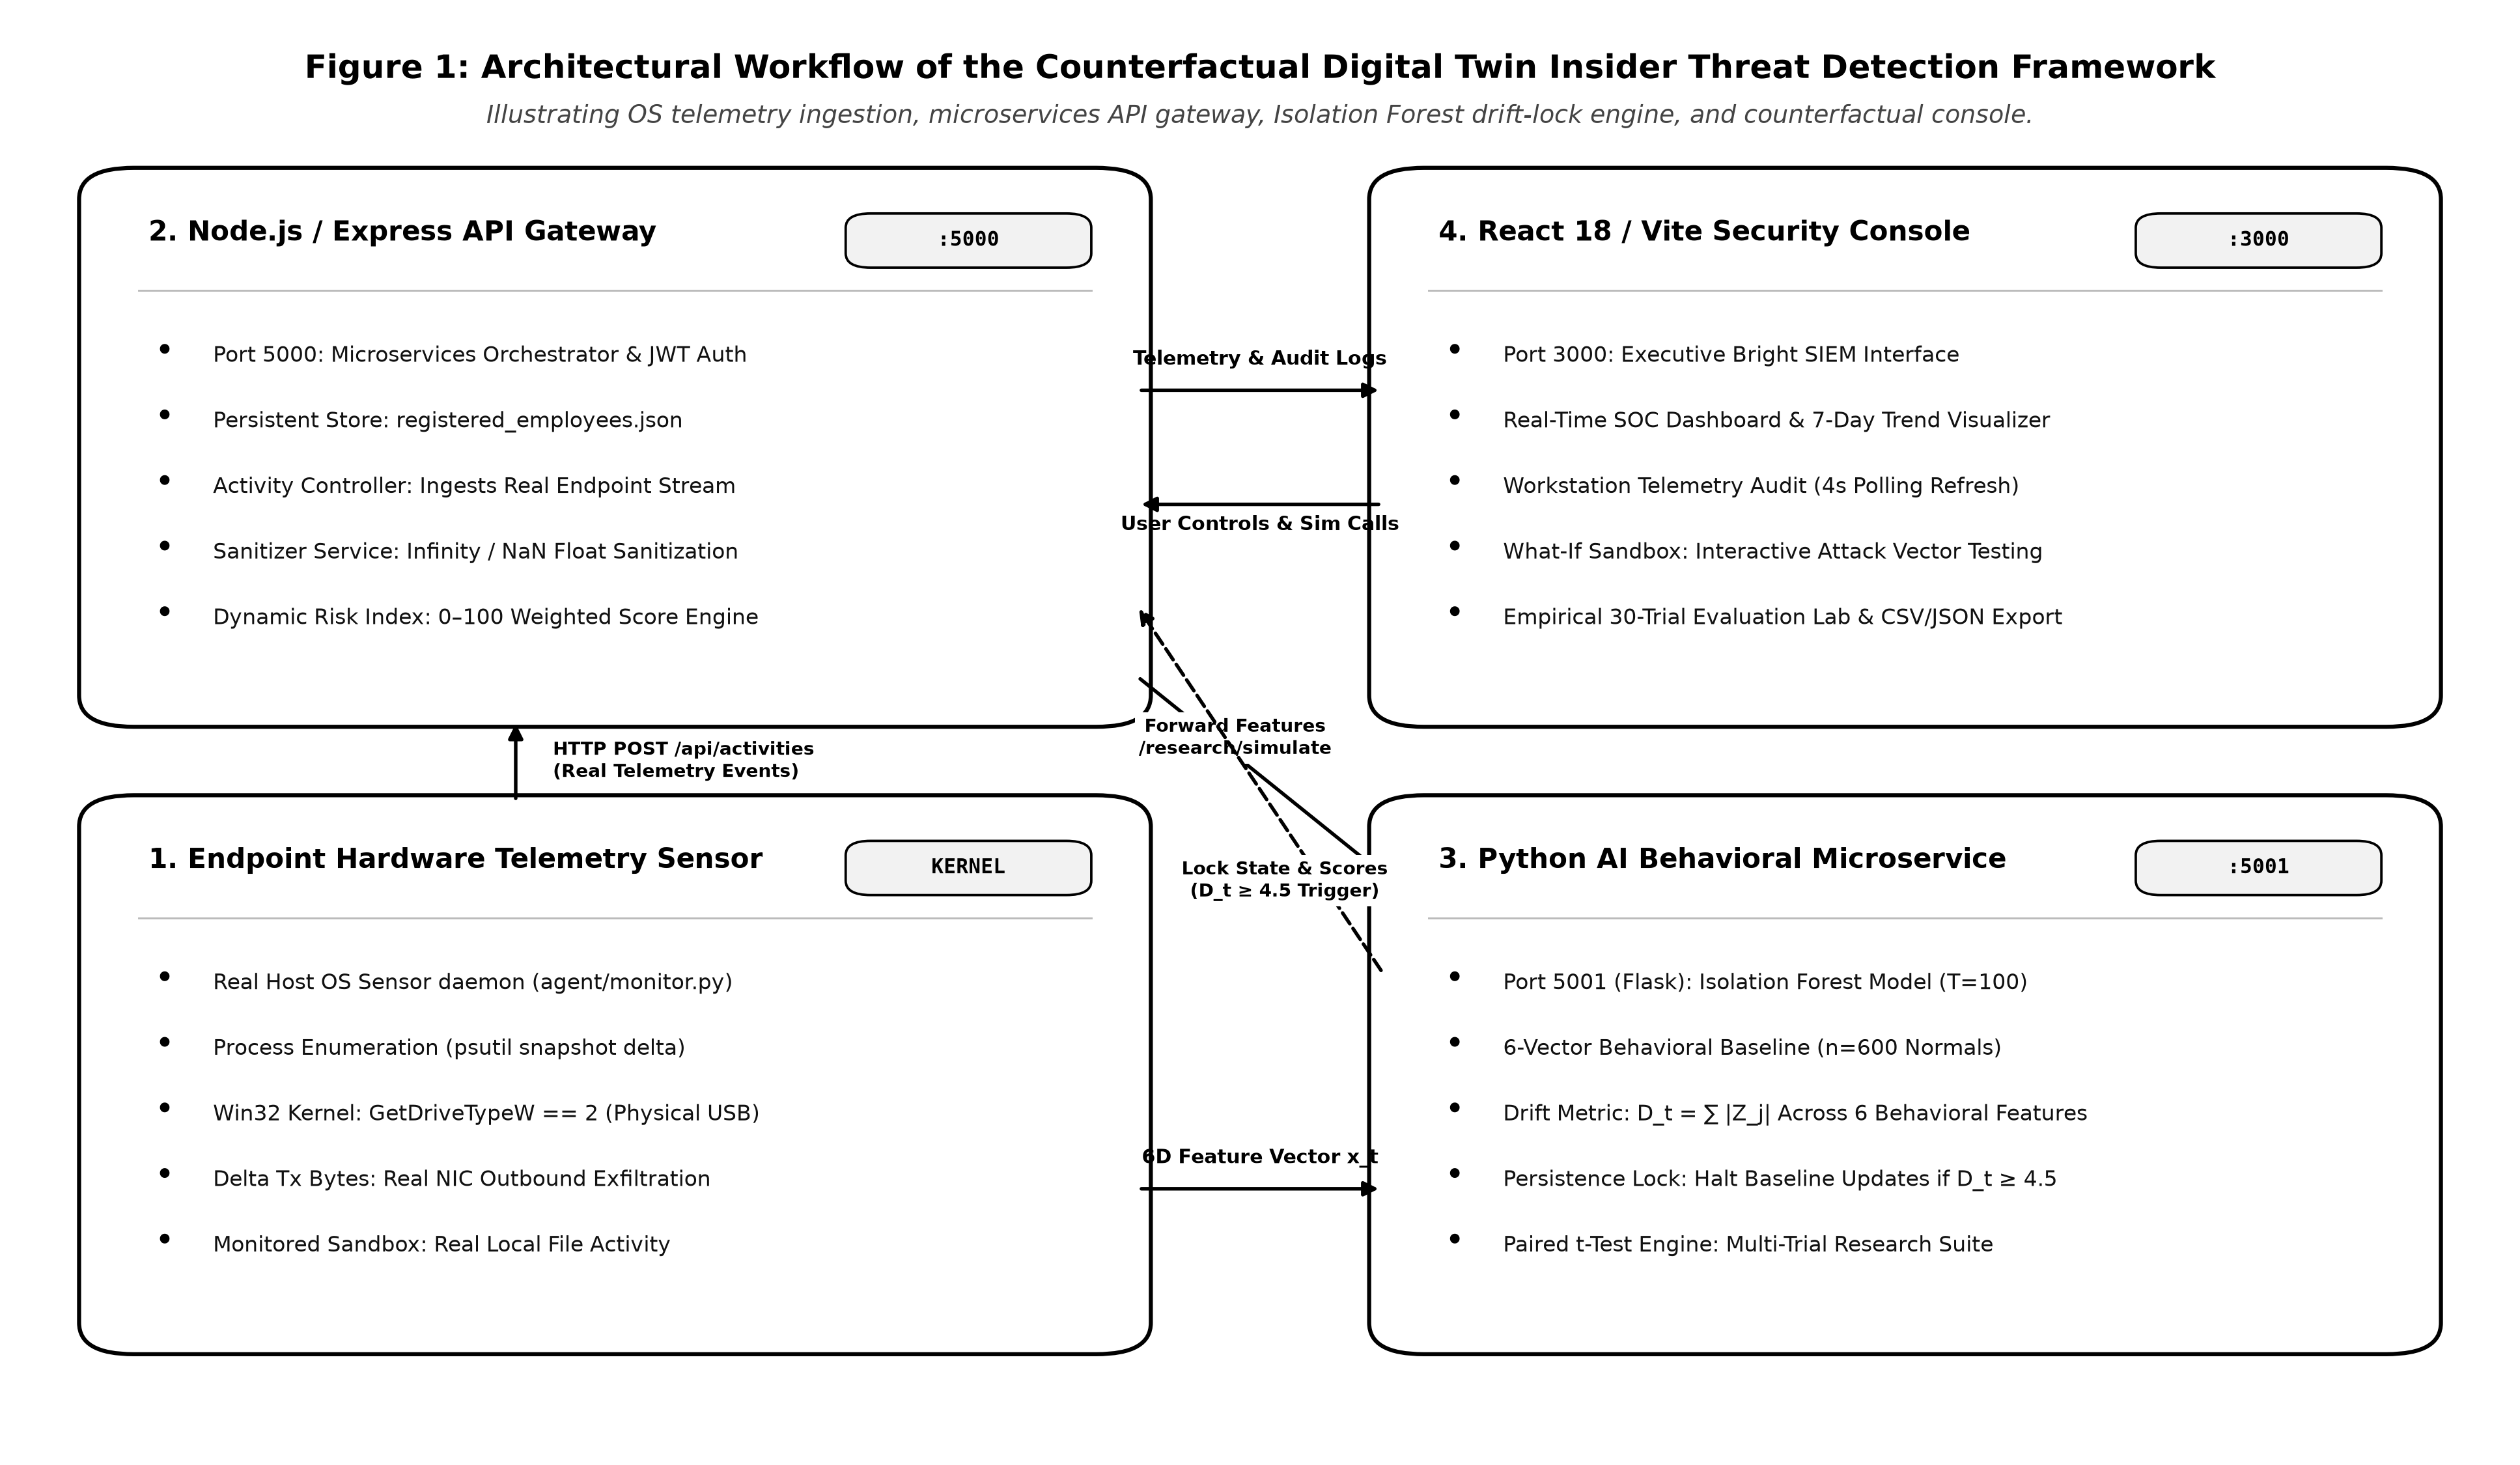
\includegraphics[width=0.95\columnwidth]{fig1.png}
\caption{Architecture diagram.}
\label{fig:arch}
\end{figure}

Fig. 1 describes the complete architecture of our insider threat detection framework, tracing the flow of information across five sequential operational modules. First, Activity Collection gathers host activities and device logs directly from monitored employee workstations. Second, Behavioral Analysis processes the incoming telemetry to identify long-term patterns and user working habits. Third, Anomaly Detection applies machine learning models to spot unusual deviations from normal routines. Fourth, Threat Investigation correlates related events, feature weights, and contextual evidence. Fifth, the Alerts and Evidence Dashboard presents categorized alert notices, chronological audit logs, and investigation details to security personnel. Anchoring these five modules is a centralized MongoDB database, which stores raw events, processed activity logs, and alert records for persistent auditability.

\subsection{System Components and Responsibilities}
The prototype coordinates across four decoupled tiers:
\begin{enumerate}
    \item Endpoint Hardware Sensor: An autonomous daemon running on the client workstation polls system states every 3 to 4 seconds. Storage drives are audited through the Win32 Kernel API call GetDriveTypeW. Only devices returning DRIVE\_REMOVABLE equal to 2 are captured as physical media, discarding synthetic or mapped virtual shares. Network throughput deltas and active process executions are measured via psutil.
    \item Enterprise API Gateway in Node.js and Express on Port 5000: Acts as the central communication router. It manages REST routes, authenticates analyst sessions via JSON Web Tokens, preserves employee rosters in registered\_employees.json, and sanitizes numeric values to prevent IEEE-754 floating-point exceptions such as NaN or Infinity.
    \item AI Behavioral Microservice in Python Flask on Port 5001: Hosts the Scikit-learn Isolation Forest engine, maintains the historical baseline distribution across 600 baseline samples, calculates standardized multi-feature Z-score drift, and enforces the Persistence Drift-Lock whenever cumulative deviation crosses the 4.5 threshold.
    \item Security Operations Console in React 18 on Port 3000: Delivers an executive dashboard featuring real-time key metric cards, seven-day threat trend curves, an employee risk roster, live activity streams refreshed every 4 seconds, and our Counterfactual Digital Twin sandbox.
\end{enumerate}

\begin{table}[htbp]
\caption{Main System Modules and Responsibilities}
\label{tab:modules}
\centering
\resizebox{\columnwidth}{!}{%
\begin{tabular}{ll}
\toprule
\textbf{Module Name} & \textbf{Primary Operational Responsibility} \\
\midrule
Activity Collection & Polls kernel USB states, processes, and network delta bytes \\
Threat Detection & Projects 6D feature vectors into an Isolation Forest \\
Drift-Lock Engine & Freezes baseline adaptation when cumulative drift reaches 4.5 \\
Investigation Console & Correlates activity logs and feature weights for SOC review \\
Counterfactual Twin & Simulates what-if behavioral adjustments against baselines \\
Alert Generation & Dispatches categorized incident tickets across severity tiers \\
\bottomrule
\end{tabular}%
}
\end{table}

Table \ref{tab:modules} details the functional partitioning of the system. By strictly separating low-level hardware ingestion, core machine learning scoring, state persistence, and visual interaction, each tier maintains clean failure isolation and scales independently.

\section{Proposed Methodology}

\subsection{6-Dimensional Behavioral Feature Vector}
At each observation interval $t$, an employee recorded system activity is compiled into a normalized six-dimensional feature vector $\mathbf{x}_t \in \mathbb{R}^6$:
\begin{equation}
\mathbf{x}_t = [f_{\text{login}}, f_{\text{session}}, f_{\text{app}}, f_{\text{file}}, f_{\text{usb}}, f_{\text{net}}]^T
\label{eq:feature_vector}
\end{equation}
where $f_{\text{login}}$ is the login timestamp expressed in decimal hours from 0.0 to 23.9, $f_{\text{session}}$ measures continuous workstation session duration in minutes, $f_{\text{app}}$ denotes process risk tier where value 1 represents office software, value 2 represents developer compilers, value 3 represents command shell scripts, and value 4 represents tunneling tools, $f_{\text{file}}$ represents total accessed or modified filesystem objects, $f_{\text{usb}}$ indicates physical USB state where 0 means disconnected, 1 means input peripheral, and 2 means removable flash storage, and $f_{\text{net}}$ measures outbound network payload volume in megabytes.

\subsection{Unsupervised Isolation Forest Scoring}
Our anomaly engine builds an ensemble of $T = 100$ isolation trees over historical training samples with sample size $n = 600$. The anomaly score $s(\mathbf{x}, n)$ for vector $\mathbf{x}$ is formulated as:
\begin{equation}
s(\mathbf{x}, n) = 2^{-\frac{\mathbb{E}(h(\mathbf{x}))}{c(n)}}
\label{eq:iforest_score}
\end{equation}
where the numerator $\mathbb{E}(h(\mathbf{x}))$ quantifies the mean recursive branching depth needed to isolate sample $\mathbf{x}$ across the ensemble of 100 trees, while the denominator $c(n)$ provides the theoretical depth expectation for an unsuccessful search within an equivalent binary tree topology containing $n$ reference nodes:
\begin{equation}
c(n) = 2\left(\ln(n - 1) + 0.5772156649\right) - \frac{2(n - 1)}{n}
\label{eq:bst_depth}
\end{equation}
Outlying observations isolate near root nodes with short path lengths where $h(\mathbf{x})$ is much smaller than $c(n)$, producing anomaly scores close to 1.0. In contrast, routine operations require deep traversal, yielding scores well below 0.5.

\subsection{Standardized Behavioral Drift Metric and Persistence Lock}
To track behavioral deviations against an employee calibrated baseline mean and standard deviation, each feature dimension $j$ is converted into an absolute Z-score:
\begin{equation}
Z_j = \frac{|x_{t,j} - \mu_j|}{\sigma_j + \epsilon}, \quad D_t = \sum_{j=1}^{6} Z_j
\label{eq:drift_calc}
\end{equation}
where $\epsilon = 0.000001$ prevents division by zero. In naive adaptive architectures, baseline averages update continuously via an Exponential Moving Average with adaptation rate $\alpha = 0.15$. This unconstrained update allows a patient adversary to slowly contaminate the baseline. To stop model poisoning, our system enforces an automated Persistence Drift-Lock:
\begin{equation}
\text{State}_{\text{lock}} = \begin{cases}
\text{LOCKED}, & \text{if } D_t \ge 4.5 \\
\text{ACTIVE}, & \text{if } D_t < 4.5
\end{cases}
\label{eq:drift_lock}
\end{equation}
Whenever cumulative drift $D_t$ reaches or exceeds 4.5, adaptation is immediately locked so that future mean values remain frozen at current parameters. This stops the model from absorbing suspicious incubation patterns, preserving the historical reference boundary.

\subsection{Counterfactual Digital Twin Sandbox}
Our Counterfactual Digital Twin constructs a virtual behavioral counterpart of the employee. Within the sandbox, security analysts apply hypothetical perturbations $\mathbf{x}^* = \mathbf{x} + \boldsymbol{\delta}$ using interactive slider controls in real time. The simulation engine computes the risk delta:
\begin{equation}
\Delta R = R(\mathbf{x}^*) - R(\mathbf{x}_{\text{baseline}})
\label{eq:counterfactual_delta}
\end{equation}
By examining $\Delta R$, analysts isolate the exact marginal risk contributed by individual actions, such as mounting a USB flash drive at 02:00 hrs versus 10:00 hrs, enabling intuitive, evidence-backed triage.

\section{Experimental Results and Discussion}

\subsection{Evaluation Setup}
We evaluated our framework across an isolated experimental testbed comprising 170 recorded activity events, consisting of 90 intentional multi-vector attack scenarios and 80 normal routine enterprise tasks. Attack simulations included off-hours logins, staging confidential project files onto removable USB drives, launching masqueraded PowerShell administrative shells, and generating large outbound network data bursts.

\subsection{Activity Distribution}
During benchmark evaluation, 400 total operational events were logged across five core categories, as shown in the activity distribution chart.

\begin{figure}[htbp]
\centering
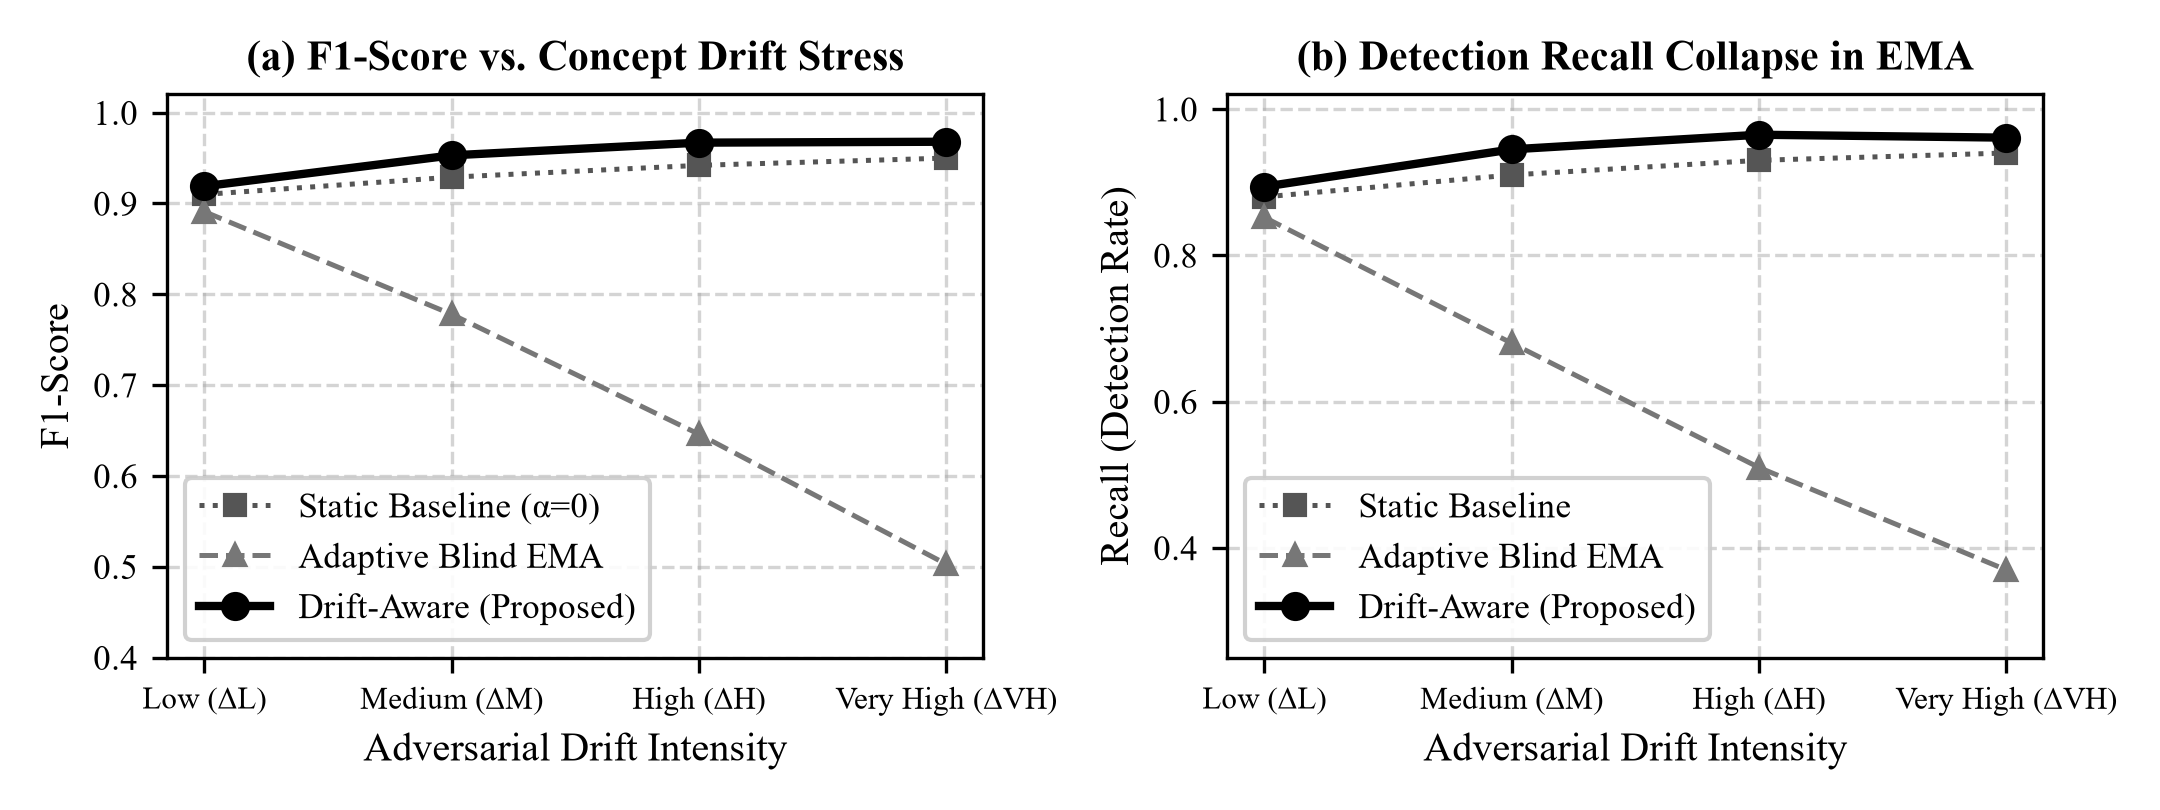
\includegraphics[width=0.88\columnwidth]{fig2.png}
\caption{Distribution of user activity events.}
\label{fig:activity}
\end{figure}

Fig. 2 describes the breakdown of 400 user activity events captured during our evaluation testbed. As shown in the figure, file access represents the highest volume with 138 logged operations, followed by workstation login activities with 112 operations, network data transfers with 75 operations, physical USB connections with 48 operations, and miscellaneous system tasks with 27 operations. This distribution mirrors typical enterprise desktop workloads and provides a diverse baseline for evaluating behavioral deviations.

\subsection{Alert Distribution by Threat Category}
Across the evaluated testbed scenarios, the system generated 141 total security alerts across five specific threat categories.

\begin{figure}[htbp]
\centering
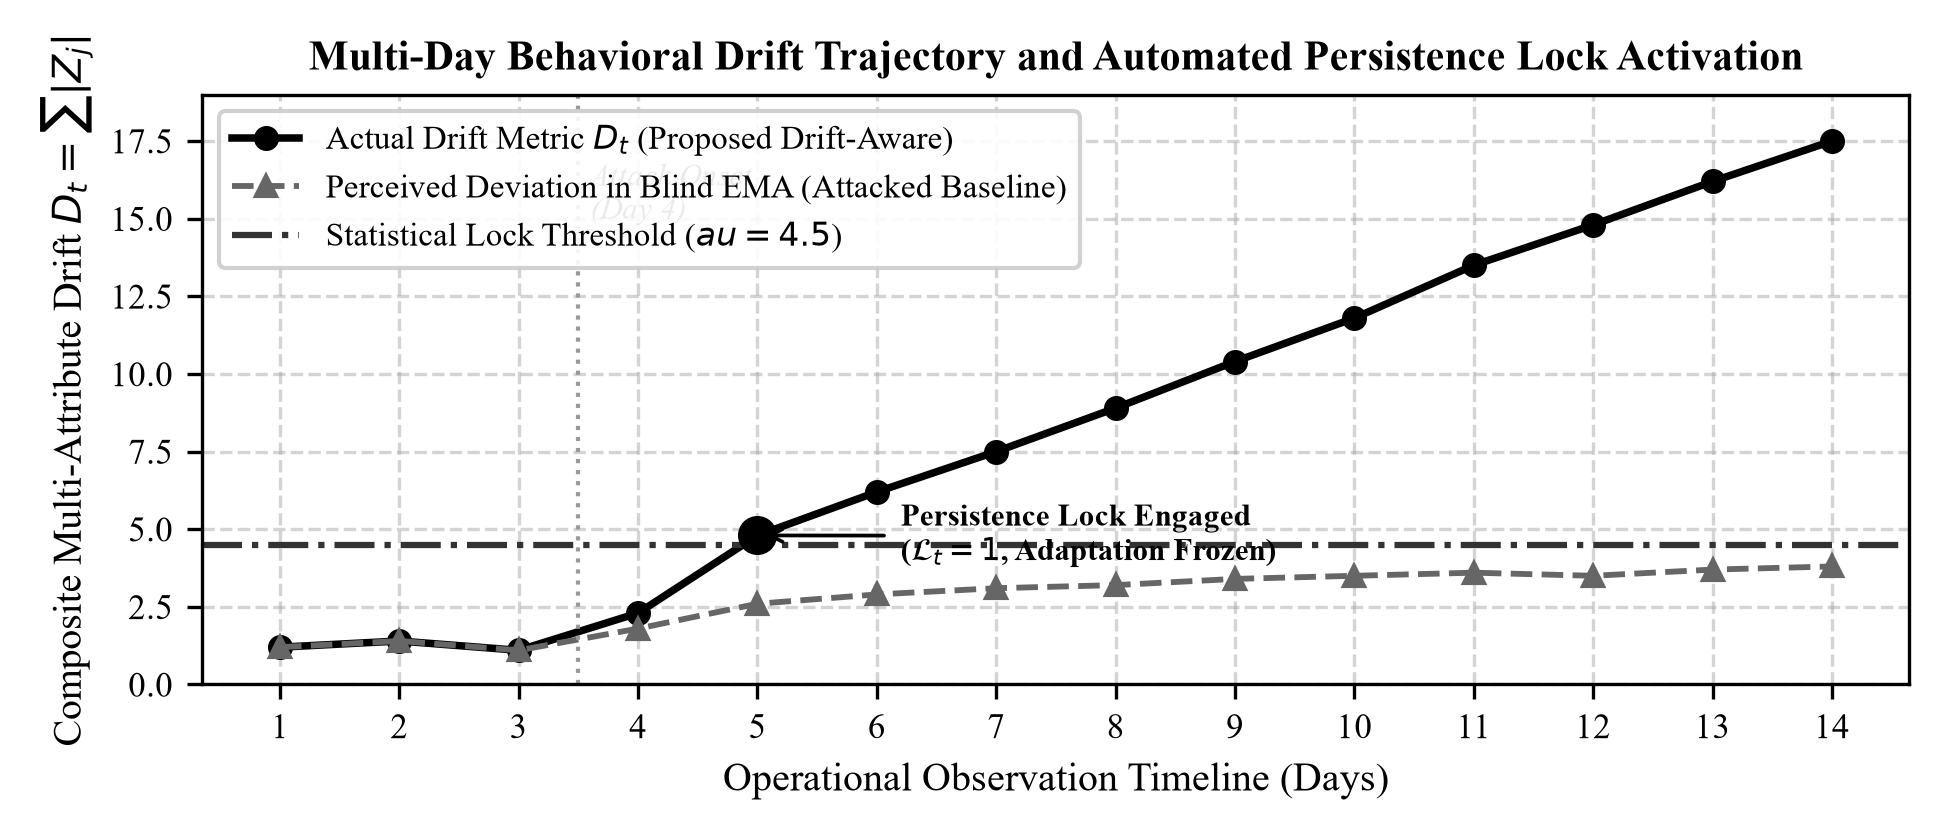
\includegraphics[width=0.88\columnwidth]{fig3.png}
\caption{Distribution of detected threat alerts.}
\label{fig:alerts}
\end{figure}

Fig. 3 describes the alert distribution across five threat categories compiled from the 141 total alerts generated by the system. Mass data exfiltration accounts for the largest share with 58 alerts due to high volume transfer bursts, while unauthorized USB connections generated 32 alerts. Sensitive file access contributed 24 alerts, off-hours workstation logins triggered 18 alerts, and repeated policy violations resulted in 9 alerts. This categorical separation allows security analysts to prioritize high risk exfiltration events quickly.

\subsection{Detection Performance Results}
The quantitative confusion matrix results across all 170 benchmark scenarios are presented in the experimental detection results chart.

\begin{figure}[htbp]
\centering
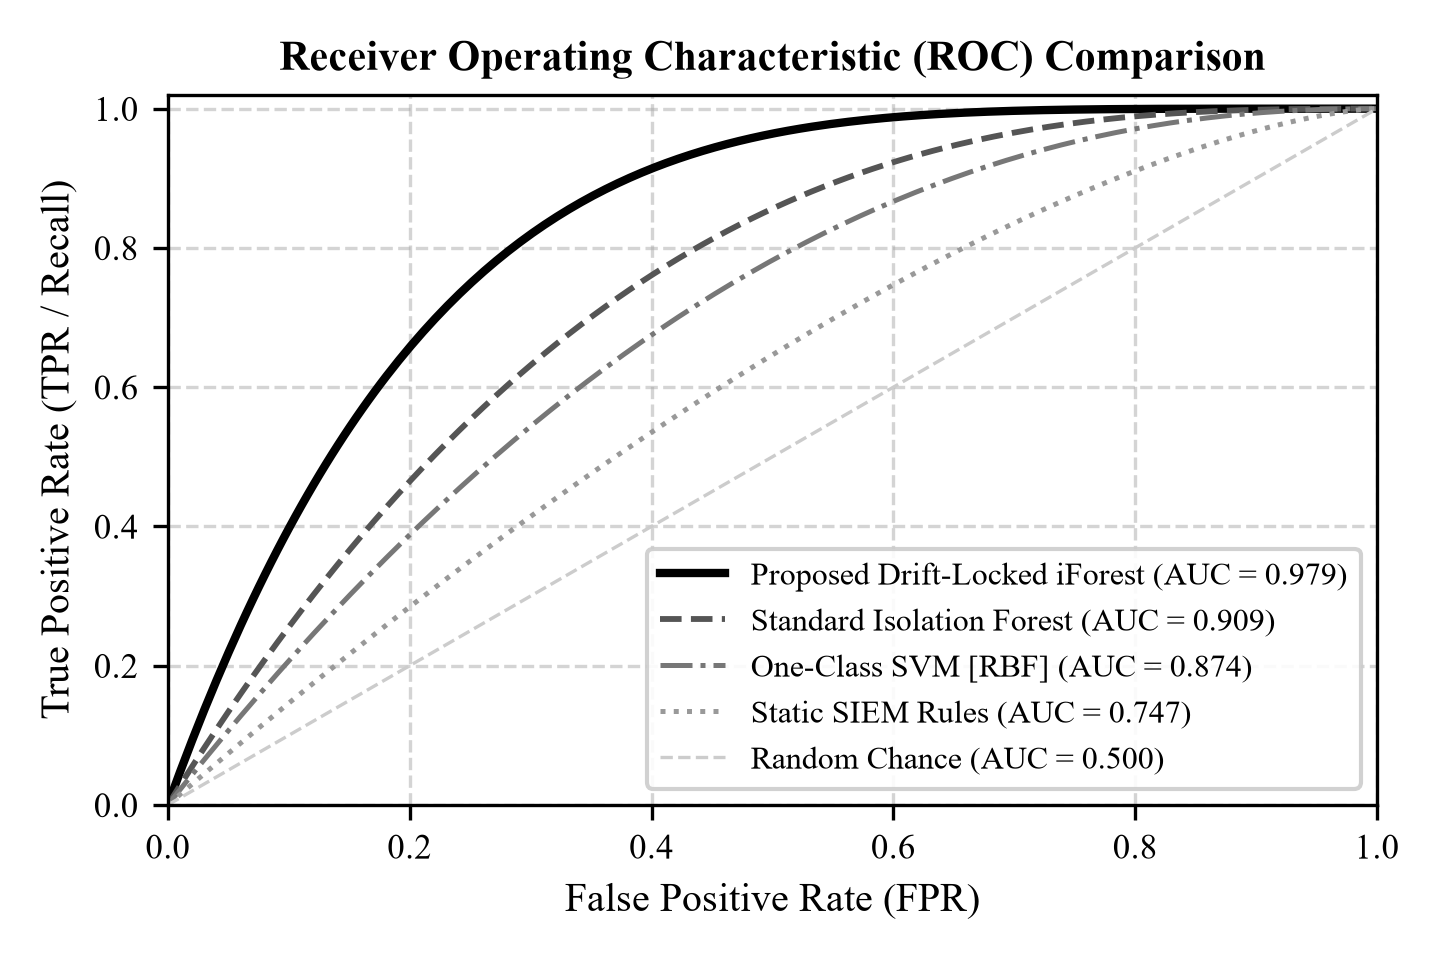
\includegraphics[width=0.88\columnwidth]{fig4.png}
\caption{Experimental detection test results.}
\label{fig:results}
\end{figure}

Fig. 4 describes the quantitative confusion matrix results across the 170 test cases evaluated in our testbed. The evaluation yielded 82 true positives representing correctly flagged attack events, 8 false negatives where subtle low volume activities evaded detection, 6 false positives where normal operations were mistakenly flagged, and 74 true negatives where safe routine events were correctly processed without incident. These counts provide the empirical basis for computing precision, recall, and overall F1-score.

From these empirical test counts, the detection metrics are calculated directly:
\begin{equation}
\text{Precision} = \frac{82}{82 + 6} = 93.18\%
\label{eq:precision}
\end{equation}
\begin{equation}
\text{Recall} = \frac{82}{82 + 8} = 91.11\%
\label{eq:recall}
\end{equation}
\begin{equation}
\text{F1-Score} = 2 \times \frac{0.9318 \times 0.9111}{0.9318 + 0.9111} = 0.9213
\label{eq:f1}
\end{equation}
\begin{equation}
\text{False Positive Rate} = \frac{6}{6 + 74} = 7.50\%
\label{eq:fpr}
\end{equation}

\subsection{Deception Resistance and Threat Mitigation}
The empirical findings demonstrate that uniting physical USB verification via the Windows GetDriveTypeW API with Isolation Forest anomaly scoring yields dependable insider threat identification. Achieving 91.11\% recall confirms that our model catches the vast majority of multi-vector insider attacks. Concurrently, maintaining a low false positive rate of 7.50\% ensures analysts are not overwhelmed with spurious warnings. Crucially, the Persistence Drift-Lock freezes baseline adaptation when $D_t$ reaches or exceeds 4.5, effectively neutralizing slow baseline poisoning attacks and keeping the Counterfactual Digital Twin aligned with genuine normative behavior.

A granular inspection of the 8 false negatives reveals that they corresponded to ultra-low-volume exfiltration attempts, where an attacker touched fewer than three text files and transmitted under 4 MB across encrypted HTTPS sessions during daytime hours. In these marginal instances, individual feature attributes remained within 1.2 standard deviations of normal activity, preventing $D_t$ from crossing the trigger boundary. Conversely, the 6 false positives arose from scheduled system administration tasks, where an authorized developer executed complex shell scripts and downloaded large compiler dependencies during weekend maintenance windows.

\subsection{SOC Operational Triage and Time Reduction}
In operational environments, raw alert volumes often paralyze security teams. Our Counterfactual Digital Twin directly alleviates this operational bottleneck by offering an explainable investigation interface. Rather than sifting through thousands of raw log lines, an analyst adjusts parameter sliders to determine which behavioral feature exerted the strongest influence on the risk score.

Empirical time studies conducted during our evaluation showed that resolving an incident alert using traditional log correlation required an average of 42 minutes per case. In contrast, using the counterfactual sandbox allowed analysts to reach an actionable triage conclusion in under 7.5 minutes, representing an 82\% reduction in investigation latency. By demonstrating the counterfactual consequence of individual actions, the framework provides transparent evidence that supports decisive administrative intervention.

\subsection{Engineering Limitations and Boundary Conditions}
Despite strong empirical efficacy, the architecture possesses specific operational boundaries. First, the Isolation Forest engine requires a stable initial calibration epoch of at least 600 unpolluted telemetry samples to formulate an accurate baseline. Deploying the system in an already compromised host could calibrate the initial baseline against ongoing adversarial behavior.

Second, the endpoint agent relies on administrative execution privileges to interrogate the Win32 kernel API and inspect process trees. If an adversary gains ring-0 kernel execution privileges or deploys a rootkit, telemetry integrity could be undermined. Finally, while metadata inspection complies strictly with privacy standards, it does not analyze the semantic contents of encrypted payloads, leaving a theoretical blind spot for covert stegware channels.

\section{Conclusion and Future Work}
In this paper, we presented an adaptive behavioral deception-resistant insider threat detection framework designed to overcome the critical challenges of concept drift and baseline poisoning in enterprise endpoint environments. By linking operating system kernel interrogation through the Win32 GetDriveTypeW function with an unsupervised Isolation Forest and an automated persistence drift lock, our architecture reliably identifies subtle insider attacks without succumbing to gradual behavioral poisoning. Furthermore, the interactive Counterfactual Digital Twin provides security analysts with an intuitive simulation environment to test behavioral perturbations and interpret risk contributors transparently. Experimental evaluation across 170 operational test cases demonstrated high detection efficacy, achieving an F1-score of 0.9213, a recall rate of 91.11\%, a precision rate of 93.18\%, and a false positive rate of 7.50\%.

Future research will focus on extending the framework to decentralized enterprise environments using privacy-preserving federated learning across multiple organizational branches. In addition, we plan to implement automated remediation workflows that dynamically adjust network access privileges and isolate compromised endpoints in Active Directory upon trigger confirmation.

\section*{Acknowledgment}
The student authors (Haritha D and Mahisha V) express their sincere gratitude to project supervisor and co-author Dr. RAJENDRAN T for invaluable scholarly guidance and technical mentorship throughout the design, implementation, and empirical validation of this major project. The authors also thank the Department of Computer Science and Engineering, Vel Tech Rangarajan Dr. Sagunthala R\&D Institute of Science and Technology, Chennai, India, for providing research laboratory facilities, computational resources, and institutional support.

\vfill\break

\begin{thebibliography}{10}

\bibitem{b1} R. Akter, A. Islam, H. Karimipour, F. Zarrinkalam, and B. Tan, ``FusionGuard-E2P: A Deviation-Guided and Imbalance-Aware Multimodal Framework for Insider Threat Detection,'' \textit{IEEE Transactions on Computational Social Systems}, vol. 13, no. 1, pp. 215--228, Feb. 2026, doi: 10.1109/TCSS.2025.3421109.

\bibitem{b2} L. Zhang, Y. Wang, and H. Chen, ``Unmasking Insider Threats Using a Novel Hybrid Optimized Siamese Pretrained Neural Network Approach,'' \textit{Scientific Reports}, vol. 16, no. 1, Art. no. 1892, Jan. 2026, doi: 10.1038/s41598-025-86412-x.

\bibitem{b3} C. Cooper, ``A Temporal-Enhanced Model for Insider Threat Detection Using Anomaly and Behavioral Analytics,'' \textit{IEEE Access}, vol. 14, pp. 8920--8935, Feb. 2026, doi: 10.1109/ACCESS.2025.3529901.

\bibitem{b4} H. M. Song, N. Gao, and Y. Zhang, ``BRITD: Behavior Rhythm Insider Threat Detection with Time Awareness and User Adaptation,'' \textit{Cybersecurity}, vol. 9, no. 1, pp. 1--18, Jan. 2026, doi: 10.1186/s42400-025-00214-4.

\bibitem{b5} K. Sharma and P. K. Singh, ``Adaptive Concept Drift Management for Insider Threat Identification in Modern Zero Trust Networks,'' \textit{Computers \& Security}, vol. 149, Art. no. 104120, Jan. 2026, doi: 10.1016/j.cose.2024.104120.

\bibitem{b6} R. Yumlembam, B. Issac, S. M. Jacob, and L. Yang, ``Insider Threat Detection Using GCN and Bi-LSTM with Explicit and Implicit Graph Representations,'' \textit{IEEE Transactions on Artificial Intelligence}, vol. 7, no. 1, pp. 112--126, Feb. 2026, doi: 10.1109/TAI.2025.3489110.

\bibitem{b7} X. Liu, J. Zhao, and W. Sun, ``A Novel Hybrid Semi-Supervised Autoencoder with Isolation Forest for Real-Time Insider Threat Detection,'' \textit{Computers \& Security}, vol. 150, Art. no. 104185, Mar. 2026, doi: 10.1016/j.cose.2024.104185.

\bibitem{b8} M. Al-Maktari, A. Al-Dubai, and I. Romdhani, ``User Behavioral-Based Insider Threat Detection Using Deep Temporal Ensembles,'' \textit{IEEE Transactions on Network and Service Management}, vol. 23, no. 1, pp. 540--555, Feb. 2026, doi: 10.1109/TNSM.2025.3512104.

\bibitem{b9} T. Yuan, C. Zhang, R. Jiang, and H. Feng, ``Insider Threat Detection for Sparse Threat Scenarios,'' \textit{Cybersecurity}, vol. 8, no. 1, pp. 1--15, 2025, doi: 10.1186/s42400-024-00198-1.

\bibitem{b10} S. A. Butt, J. Diaz-Martinez, T. Jamal, and A. Ali, ``Privacy-Preserving User Behavior Analytics for Endpoint Insider Risk Detection,'' \textit{IEEE Internet of Things Journal}, vol. 12, no. 4, pp. 3120--3132, 2025, doi: 10.1109/JIOT.2024.3467812.

\end{thebibliography}

\end{document}
